% !TEX root = flow_head.tex
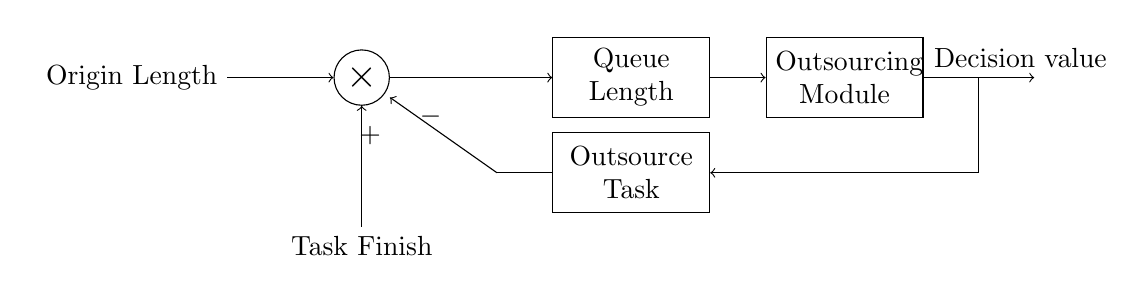
\begin{tikzpicture}[node distance=5mm and 5mm,
square/.style={
% The shape:
rectangle,
draw=black,
minimum size=2.9em,
text width=5em,
text centered
},
coord/.style={
coordinate,
% on chain,
% on grid,
% node distance=6mm and 25mm
},
circle/.style={
rectangle,minimum size=2em,rounded corners=1em,
draw=black
},
skip loop/.style={to path={-- ++(0,#1) -| (\tikztotarget)}}
]
\matrix[row sep=0.5em,column sep=2em] {
% First row:
\node (origin) {Origin Length} ; & \node (compare) [circle] {\Large$\times$}; & & \node (length) [square] {Queue Length} ; & \node (outsource) [square] {Outsourcing Module} ; & \node (node) [coord] {} ; & \node (end) [coord] {}; \\
& & \node (p1) [coord] {} ; & \node	(out) [square] {Outsource Task} ; & & & \\
& \node (tf) {Task Finish}; & & & & &\\
};
\path (origin) edge[->] (compare) (tf) edge[->] (compare) (compare) edge[->] (length) (length) edge[->] (outsource) (outsource) edge[->] (end);
\path (out) edge (p1) (p1) edge[->] (compare);
\draw [->] (node) |- (out) ;
\path (tf) to node [near end,xshift=0.3em] {$+$} (compare) (p1) to node [near end,xshift=0.5em] {$-$} (compare) (outsource) to node [yshift=0.7em,xshift = 1.5em] {Decision value} (end);
\end{tikzpicture}